\chapter{Playing the game: I/O in Haskell}
\chapstart

\label{io}


This chapter completes the design and implementation of the Rock - Paper - Scissors game. We start by looking at how \emph{strategies} can be represented as functions. One of the real strengths of Haskell is to be able to treat functions just like any other data, and strategies are the first time we do that in practice.
 
Next we explore how the simplest kinds of programs, reading and writing
to a terminal, can be developed in Haskell. The model we describe forms
the foundation for more complex interactions like those in a mail system
or an operating system. We start by discussing how in the past I/O has been a problem for the
users of a functional language. 
The solution in Haskell is to 
introduce the types \texttt{IO a}, which we can
think of as \emph{programs} that do some input/output before returning a value
of type \texttt{a}. These programs include simple operations to read and write
information, as well complex programs which are built from a number of 
\texttt{IO} programs
sequenced into one by means of the \texttt{do} construct. 

We conclude the chapter by explaining how to play the Rock - Paper - Scissors game: we show how to play one strategy against another, as well as how you can play interactively against a strategy.

\section{Rock - Paper - Scissors: strategies}
\label{strategiesRPS}\index{Rock - Paper - Scissors|(}

\begin{wrapfigure}[8]{r}{5cm}
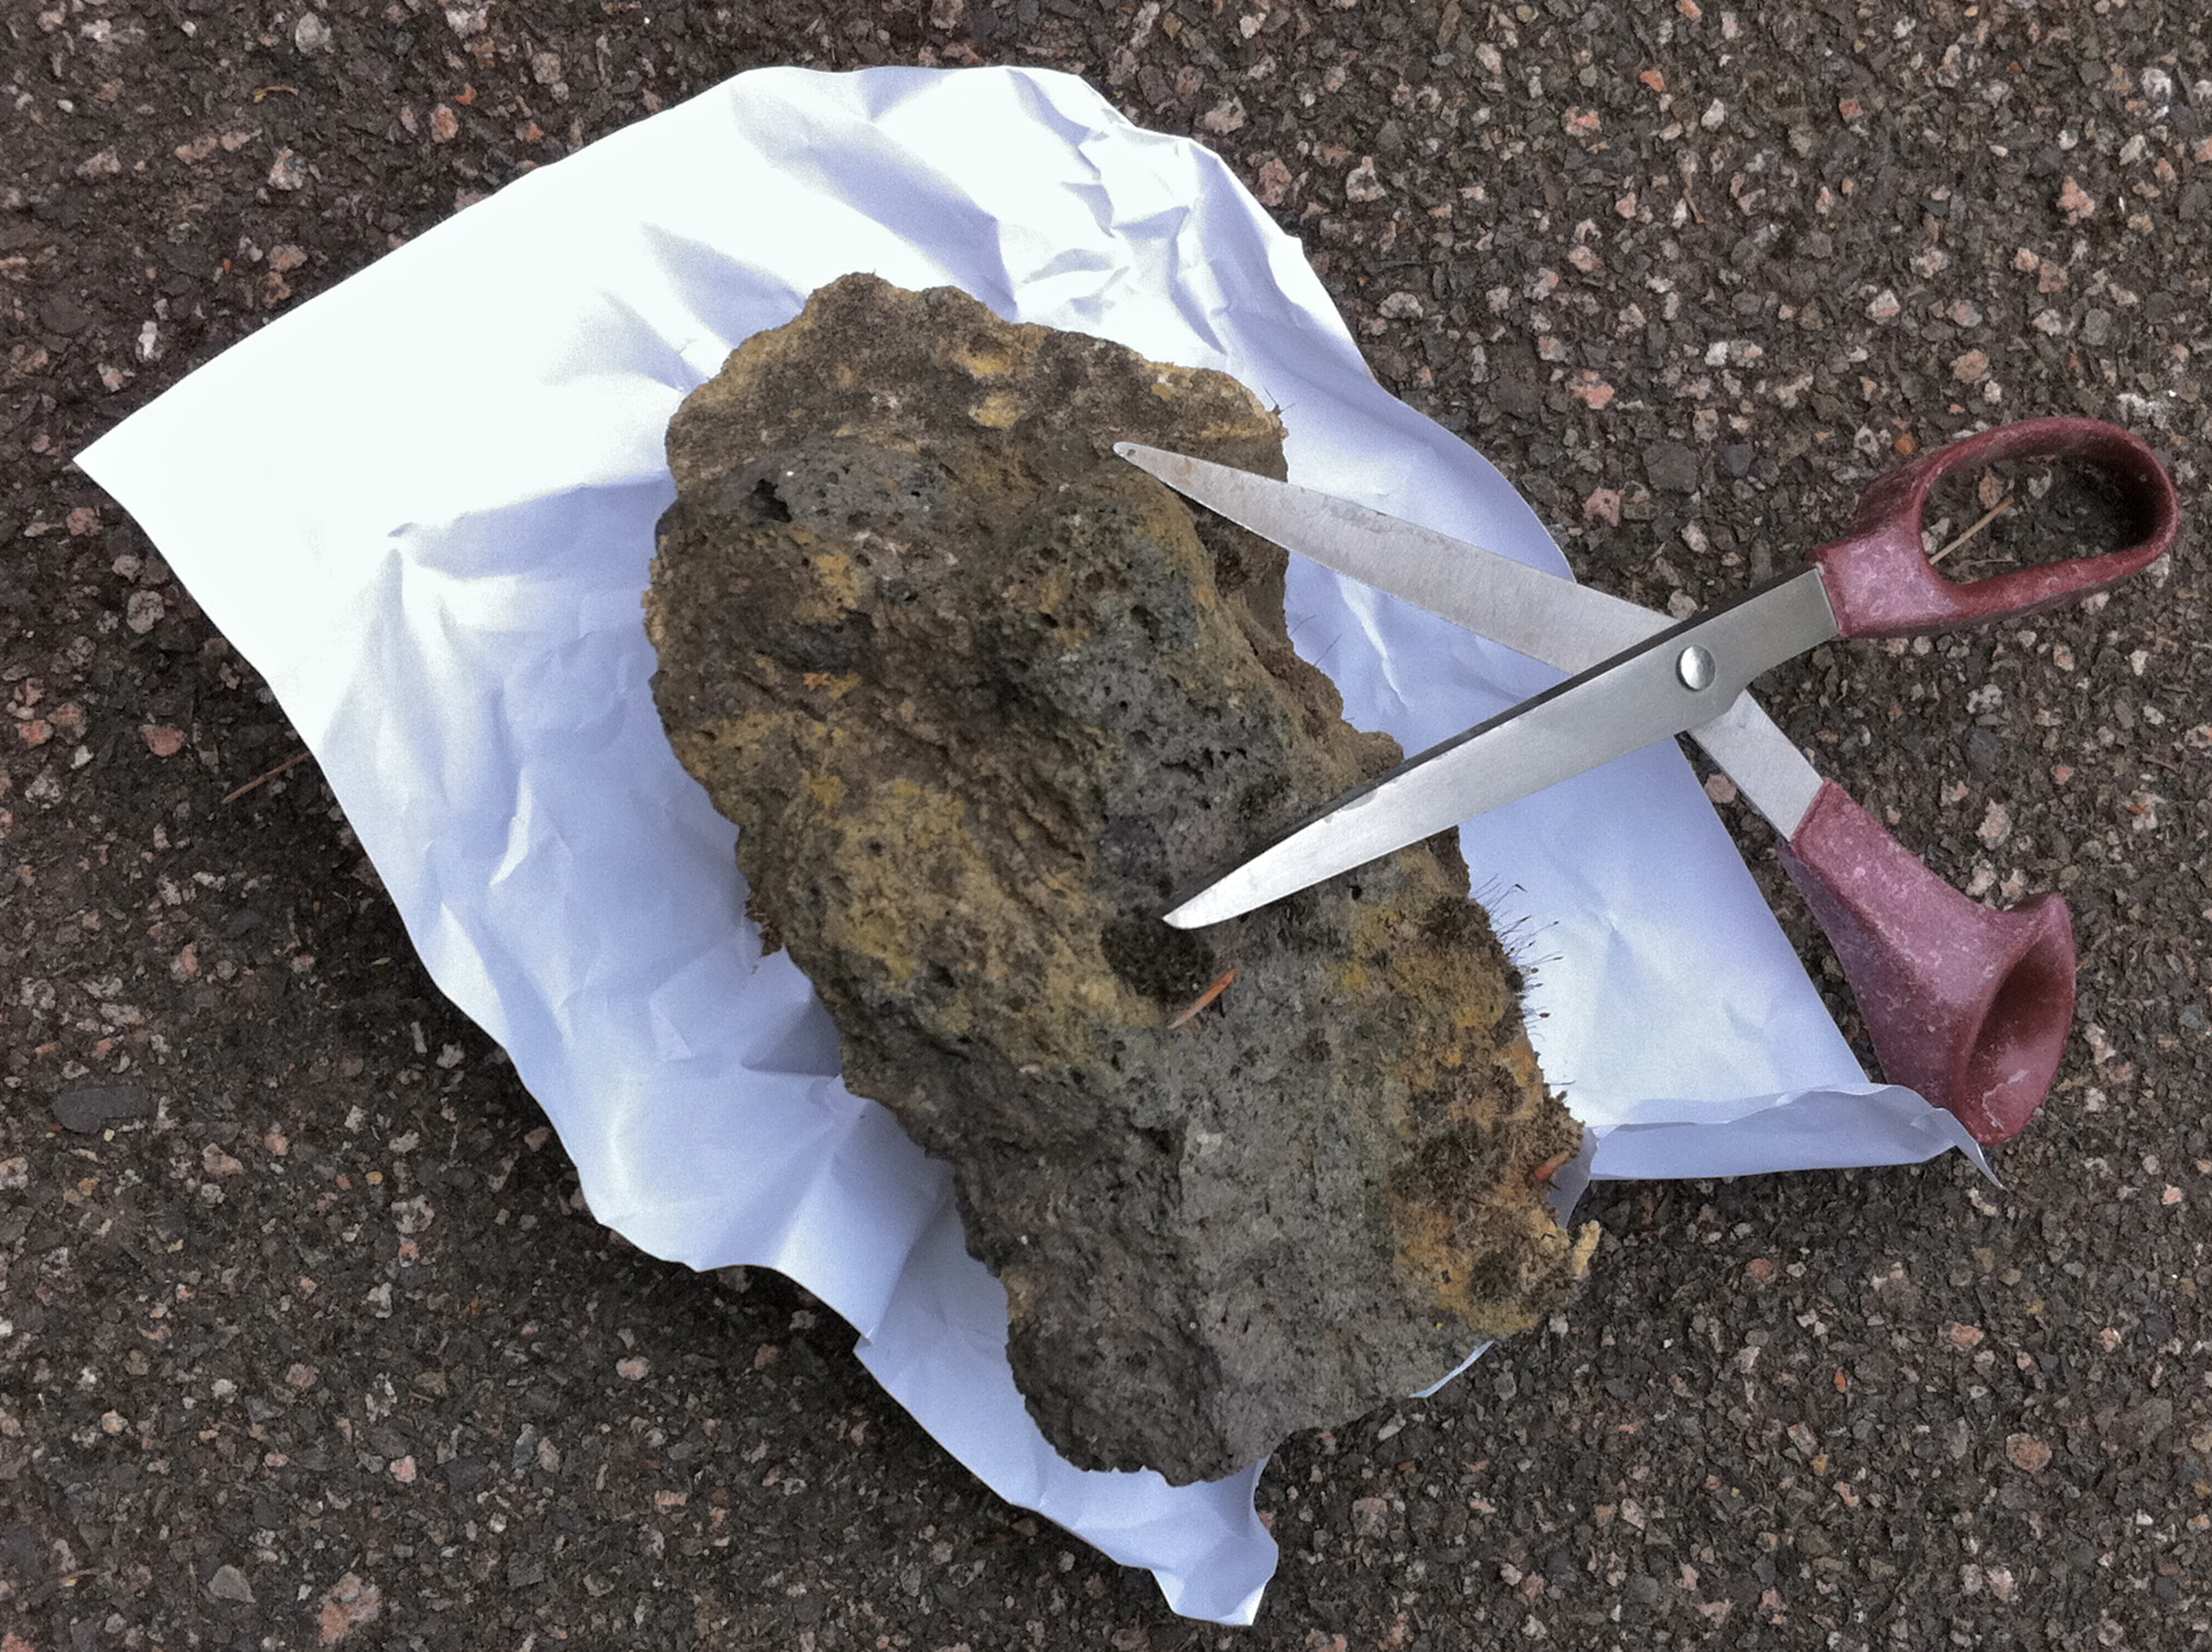
\includegraphics[width=5cm]{Pictures/RPS.pdf}
\end{wrapfigure}
Now that we have seen how to define functions over lists from scratch, as well as making use of functions in the prelude and other libraries, it is time to go back to the discussions of games that we started earlier in the book. In particular, we go back to the Rock - Paper - Scissors game, first introduced in Section \ref{EnumTypes}.

\subsection*{Scoring the moves}

Recall that we defined the \texttt{Move} type like this
\begin{alltt}
data Move = Rock | Paper | Scissors 
            deriving (Show,Eq) 
\end{alltt}
It's worth looking back at that section for definitions of the functions \texttt{beat} and \texttt{lose} as well as the type \texttt{Result} and the function \texttt{outcome} defined in the exercises. 

In that section we were concerned with a single move, but here we want to look at a whole \emph{tournament}, when two players play a sequence of moves against each other.
We can model a tournament by this type definition
\begin{alltt}\minx{Tournament}
type Tournament = ([Move],[Move])
\end{alltt}
where the lists model the moves made by the two players: let's call them A and B. An example tournament is given by
\begin{alltt}
([Rock,Rock,Paper],[Scissors,Paper,Rock])
\end{alltt}

\begin{exercises}

\item
Define a function \label{outcome}
\begin{alltt}
outcome :: Move -> Move -> Integer
\end{alltt}
which gives the outcome as 1, 0, or -1 according to whether the first \texttt{Move} beats, draws with or loses against the second \texttt{Move}. For example, we expect that 
\begin{alltt}
outcome Rock Scissors = 1
\end{alltt}

\item
Using the function \texttt{outcome} that you defined in the previous exercise, define a function
\begin{alltt}
tournamentOutcome :: Tournament -> Integer
\end{alltt}
which gives the outcome of a tournament, giving positive scores to player A, the first player. For example, we should expect
\begin{alltt}
tournamentOutcome ([Rock,Rock,Paper],[Scissors,Paper,Rock]) = 1
\end{alltt}
because the scores for the three rounds are 1, -1 and 1, summing to 1.

\end{exercises}

\subsection*{Strategies}

\index{strategies}

Suppose we want to build a program to play Rock - Paper - Scissors against an opponent. We need to find a way to describe how the machine should play, let's call this a \emph{strategy}. 

We can describe a strategy in words: something like "echo the last move" but that's not a program. Instead we can describe it as a \textbf{function}: the next move that I will play will depend (potentially) on all the moves that my opponent has played, so we can say
\begin{alltt}\minx{Strategy}
type Strategy = [Move] -> Move
\end{alltt}
Remember that \texttt{Strategy} is just shorthand for \texttt{[Move] -> Move}, so when we talk about strategies we are talking about functions that take a list of moves and return a single  `next' move. Let's take a look at some particular strategies now.


\begin{description}

\item[Constant strategy.]
The simplest way of playing is always to play the same thing! So, as strategies we have
\begin{alltt}
rock, paper, scissors :: Strategy 

rock _     = Rock
paper _    = Paper
scissors _ = Scissors
\end{alltt}
Each of these functions ignores its argument and returns the same move in every situation: it should be pretty easy to beat this once an opponent realises what's going on.

\item[Cycle through the possibilities.]
Another option is to cycle through the three possibilities in turn. One way of programming that strategy is this:
\begin{alltt}
cycle :: Strategy

cycle moves
  = case (length moves) `rem` 3 of 
      0 -> Rock
      1 -> Paper
      2 -> Scissors
\end{alltt}
How does this work? We look at the number of moves made so far, which is given by \texttt{length moves}; the remainder on dividing this by 3 cycles through 0, 1, 2 and we use a \texttt{case} expression to map these results to the three options \texttt{Rock}, \texttt{Paper}, \texttt{Scissors}.

\item[A random choice.]
We can make a random choice of play. 
\begin{alltt}
randomStrategy :: Strategy
\end{alltt}
This isn't really a proper function, in fact, because it doesn't always return the same result, we should program this using monads, as described in Chapter \ref{actions}. However, a little bit of `under the hood' work allows us to fake this in Haskell; the details are in the code for this chapter. We'll discuss the full implementation in Section \ref{furtherIO}.

\item[Echo the last move.]\label{echoStrat}
Given the list of moves made by our opponent, it's easy to play by echoing their last move. However, we have to think about one thing first: how are the moves listed in the list of moves: it could be `latest first', or `oldest first'. It's actually convenient to choose \textbf{latest first}, so that the list of moves
\begin{alltt}
[Rock,Rock,Paper]
\end{alltt}
says that \texttt{Paper} was played first, followed by two \texttt{Rock} moves. With this settled we can define the `echo' strategy:
\begin{alltt}
echo :: Strategy

echo (latest:rest) = latest
echo []            = Rock
\end{alltt}
We've had to say what is the response when there are \textbf{no} previous moves, and here we've made the arbitrary choice of \texttt{Rock}.

\item[More strategies.]
More strategies are described in the exercises, giving you a chance to code them as functions of type \texttt{Strategy} for yourself.  

\end{description}

\beware{Using functions as data}{This is an important example, and shows something that's really distinctive about functional programming, because it uses functions to model data in a completely natural way. One way to see this is to try to model strategies \emph{without} using functions: give it a try with the examples here and also those in the exercises, and you'll see that it's not possible to do it in as general a way as functions do!

\medskip
We'll talk more about functions as data and how they can be the input to and output from  other functions, called \emph{higher-order functions} in Chapters \ref{gen2} and \ref{developingHOPs}.
}

\begin{exercises}

\item
Define a strategy which plays the move which would have won against the opponent's last move. Define a strategy which plays the move which would have \emph{lost} against the opponent's last move. Which of these do you think will be a better strategy in practice? Explain your answer.

\item
Define a strategy which plays a random choice \emph{except} when the opponent's last two moves have been the same one. In this case we guess that her next move will not be the same: how does that help? Well, if we know that she's only got two choices, we can play \emph{not to lose}. 

Take the concrete example of \texttt{Rock} being played twice by our opponent. We guess that her next move will be \texttt{Paper} or \texttt{Scissors}: what should we play? The answer is \texttt{Scissors}, because then we'll win if she plays \texttt{Paper} or draw if she also plays \texttt{Scissors}!

\item
Define a strategy which looks at the frequencies that the opponent has played the three choices. If you assume they are making random plays, then why not predict they are about to play the least frequent, and use the trick from the previous exercise to make a choice.

\item {[Harder]}
Go to the World RPS website -- see the box at the end of this section -- to find out more strategies, and try to implement them.

\item {[Harder]}
Define a function 
\begin{alltt}
alternate :: Strategy -> Strategy -> Strategy
\end{alltt}
so that the strategy given by
\begin{alltt}
alternate str1 str2
\end{alltt}
is to combine the two strategies \texttt{str1} and \texttt{str2}, using them alternately.

\item {[Hard]}
Can you write a function which will \emph{analyse} an arbitrary strategy to work out what it does? You will need to think about how to represent this result: is it a string describing what the strategy does, or something a bit less informal?

\item {[Hard]}
Can you use the facilities of QuickCheck -- described in more detail in Section \ref{qcGens} -- to help to analyse what an arbitrary strategy does?

\end{exercises}



\beware{More information about Rock - Paper - Scissors }
{In fact the choice of the first move in defining \texttt{echo} is not completely arbitrary: men are most likely to choose \texttt{Rock} first. This and lots more information about Rock - Paper - Scissors can be found at the World RPS Society website:
\begin{alltt}
http://www.worldrps.com/
\end{alltt}
} 

\index{Rock - Paper - Scissors|)}


\section{Why is I/O an issue?}
\label{ioCaution}\index{I/O|(}
\index{I/O!history}

A functional program consists of a number of definitions, such as
\begin{alltt}
val :: Integer
val = 42

function :: Integer -> Integer
function n = val + n
\end{alltt}
The effect of these definitions is to associate a fixed value with each
name; in the case of \texttt{val} the value is an integer and in the case of
\texttt{function} it is a function from integers to integers.
How is an input or an output action to fit
into this model? 

One approach, taken in Standard ML \shortcite{defsml2e} and F\# \cite{Fsharp}, for instance,
is to include operations like
\begin{alltt}
inputInt :: Integer
\end{alltt}
whose effect is to read an integer from the input; the value read in becomes the value 
given to \texttt{inputInt}.
Each time \texttt{inputInt} is evaluated it will be given a new value, 
and so it is not a fixed integer value as it ought to
be according to our original model.

Allowing this operation into our language 
may not seem to cause too big a problem, but examining the example of
\begin{alltt}
inputDiff = inputInt - inputInt\hfill(inputDiff)
\end{alltt}
shows how it has two important consequences for our model of functional programming. 
\begin{itemize}
\item Suppose that the first item input is \texttt{4}, and that the next
is \texttt{3}. Depending upon the order in which the arguments to
`\texttt{-}' are evaluated, the value of \texttt{inputDiff} will be
either \texttt{1} or \texttt{-1}.
\item More seriously, \texttt{(inputDiff.1)} breaks the model of
reasoning which we have used. Up to now we would have thought that
subtracting a value from itself would have given a result of \texttt{0}, but that is
{\em not\/} the case here. 
\itempar
The reason for this is precisely that the meaning of an expression is
no longer determined by looking only at the meanings of its parts, since we cannot 
give a meaning to
\texttt{inputInt} without knowing where it occurs in a program; as we
saw in the previous point, the first and second occurrences of
\texttt{inputInt} in
\texttt{inputDiff} will generally have different values.
\end{itemize}
As the second point shows, if we take this approach then it will be
substantially more difficult to understand the meaning of any program. 
This is because {\em any\/} definition in a
program may be affected by the presence of the I/O operations. An
example is the function
\begin{alltt}
funny :: Integer -> Integer
funny n = inputInt + n
\end{alltt}
from whose definition we can see the dependence on I/O, but potentially
any function may be affected in a similar way.

Because of this, I/O proved to be a thorny issue for functional programmers
for some considerable time, and there have been a number of attempts to find the right
model for I/O -- indeed, earlier versions of Haskell included two of
these. An illuminating history and overview of functional I/O is given in
\citeN{gordon-book}. 

In this chapter we introduce the basics of I/O using the \texttt{IO} types; Chapter \ref{actions}  describes the \emph{monadic} approach to programming which underlies I/O and other forms of interaction with the `world outside'. 

\section{The basics of input/output}
\label{basicsIO}
\index{I/O!basics|(}



In
thinking about input/output\index{input/output|see{I/O}}\index{IO|see{I/O}} 
or \textbf{I/O} it makes more sense
to think of \emph{actions happening in sequence}. For instance, first
some input might be read,
and then on the basis of that some further input might be read, or output might be 
produced. 

Haskell provides the types \texttt{IO a}\minx{IO}
of \textbf{I/O actions} of type \texttt{a}\index{action, I/O} or \textbf{I/O programs} of type
\texttt{a}. An object belonging to \texttt{IO a}
is a \emph{program} which will do some I/O and then return a value of type
\texttt{a}. Built into Haskell are some primitive I/O programs, as well
as a mechanism to sequence these I/O programs. 

One way of looking
at the \texttt{IO a} types is that they provide a small \emph{imperative
programming \index{I/O!imperative programs}
language} for writing I/O programs on top of Haskell, without compromising the functional
model of Haskell itself.\footnote{The language is unusual in that it is \emph{single assignment}, like Erlang \cite{progErlang,erlangProg}; we'll explain this when we discuss the examples.}

We start by looking at the basic \texttt{IO} capabilities built into the standard prelude, and then we look at a whole lot of examples to see how to put these components together using the
\texttt{do} notation. In the next section we look at how to write `functional loops' to form more complex I/O programs.




\subsection*{Reading input}
\index{I/O!input}

The operation which reads a line of text from the standard input does some I/O and
returns a \texttt{String} which is the line just read. According to the
explanation above, this should be an object of type \texttt{IO String}, and
indeed, the built-in function 
\begin{alltt}\minx{getLine}
getLine :: IO String\minx{getLine}
\end{alltt}
reads a line from the standard input. In a similar way, 
\begin{alltt}
getChar :: IO Char\minx{getChar}
\end{alltt}
will read a single character from the input.

\subsection*{The one-element type}
\index{type!one element}

Haskell contains the type \texttt{()}, which contains one element only.
This element is also written \texttt{()}. A value of this type can convey no useful
information  and so the type is not often used. However, it {\em is\/} useful
in performing \texttt{IO}, as there are cases of IO programs
whose only significance is their I/O actions and not the results they return.
Programs of that sort will have type
\begin{alltt}
IO ()\minx{()}
\end{alltt}
and they will return the value \texttt{()} as their result.


\subsection*{The \texttt{Main} module and the \texttt{main} program}
\minx{Main}\minx{main}

If we compile a Haskell project using GHC, the Glasgow Haskell Compiler, then this produces executable program which runs the function
\begin{alltt}
main :: IO t
\end{alltt}
for some type \texttt{t}: often this is \texttt{()}, so that
\begin{alltt}
main :: IO ()
\end{alltt}
By default, this \texttt{main} program is expected to be in the \texttt{Main} module, but it can be given in any module from the project.


\subsection*{Writing \texttt{Strings}}
\index{I/O!output}

The operation of writing the string \texttt{"Hello, World!"} will be an
object which performs some I/O, but which has nothing of significance to
pass back to the program. It is therefore of type \texttt{IO ()}. 

The general operation to print a text string will be a 
\textbf{function} which
takes the string to be written, and gives back the I/O object which writes
that string:
\begin{alltt}
putStr :: String -> IO ()\minx{putStr}
\end{alltt}
and using this we can write our `hello, world' program.
\begin{alltt}\minx{helloWorld}
helloWorld :: IO ()
helloWorld = putStr "Hello, World!"
\end{alltt}
Using \texttt{putStr} we can define a function to write a line of output.
\begin{alltt}
putStrLn :: String -> IO ()\minx{putStrLn}
putStrLn = putStr . (++ "\bs{n}")
\end{alltt}
The effect of this is to add
a newline to the end of its input before passing it to
\texttt{putStr}.

\subsection*{Writing values in general}

The Haskell prelude provides the class \texttt{Show}
with the function
\begin{alltt}\minx{Show}
show :: Show a => a -> String
\end{alltt}
which can be used to write values of many types. For example, we
can define a general print function from the standard prelude thus
\begin{alltt}\minx{print}
print :: Show a => a -> IO ()
print = putStrLn . show
\end{alltt}

\subsection*{Returning a value: \texttt{return}}
\index{I/O!returning a value}
\minx{return}

Suppose we want to write an I/O action which does no I/O but does return
a value -- we will see examples of this in due course. This is achieved 
by the built-in function
\begin{alltt}
return :: a -> IO a
\end{alltt}
The effect of \texttt{return x} is to do no I/O, but simply to return the
result \texttt{x}. 

If we're writing a program of type \texttt{IO ()} then \texttt{return ()} has the effect of a `\texttt{skip}' in a traditional language: it's a command that does nothing. We use this in cases where we only want to perform an action when a condition holds, like this:
\begin{alltt}
if condition
  then action
  else return ()
\end{alltt}




\subsection*{Running an I/O program}
\index{I/O!running a program}

We have written a simple I/O program, namely \texttt{helloWorld}; how is
it run? In GHCi we can evaluate it at the prompt:
\begin{alltt}\minx{main}
\textsl{Main>} helloWorld
\textsl{Hello, World!}
\textsl{Main>} ...
\end{alltt}
Strictly speaking, the \texttt{main} definition of a Haskell
program should be of type \texttt{IO a} for some \texttt{a}. In GHCi, if
we ask to evaluate an expression \texttt{e} of type \texttt{b}
then it is wrapped up as an object of type \texttt{IO ()} by applying
the
\texttt{print} function.
\medskip

\noindent This completes our introduction to the basic I/O functions in the standard
prelude as well as the method by which \texttt{IO} programs are run.

Next we look at how programs are sequenced, and also how to use the values read in
by means of input programs like
\texttt{getLine}; this is the topic of the next section. 
\index{I/O!basics|)}

\section{The \texttt{do} notation}
\markright{The \texttt{\runinghead do} notation}
\index{sequencing|see{\texttt{do}}}
\index{do@\texttt{do} notation}
\index{I/O!\texttt{do} notation|(}

The \texttt{do} notation gives us a way of building IO programs from the components that we discussed in the previous section. The \texttt{do} notation supports two things:
\begin{itemize}
\item
it is used to \emph{sequence} I/O programs, and
\item
it is used to \textbf{name}\footnote{or `capture' or `bind'} the values returned by \texttt{IO} actions; this means that the later actions can depend on values captured earlier in the program.
\end{itemize}
Together these ideas make a \texttt{do} expression appear like a
simple imperative program, containing a sequence of commands and
assignments; although this analogy is not complete -- we examine how it
breaks down in the next section -- it shows that the model of I/O given
by the \texttt{IO} types is a familiar one, albeit in a different guise.

\subsection*{Sequencing I/O actions}

One purpose of the \texttt{do} construct is to sequence I/O actions 
and we show how it is used through a series of examples.
\begin{example}
\subexample*{1.} 
We begin by looking at
the definition of \texttt{putStrLn} from the standard
prelude. The effect of \texttt{putStrLn str} is to do two things: first
the string \texttt{str} is output, then a newline. This is accomplished
by
\begin{alltt}\minx{putStrLn}
putStrLn :: String -> IO ()

putStrLn str = do putStr str
                  putStr "\bs{n}"
\end{alltt}
Here we see the effect of \texttt{do} is to sequence a number of
\texttt{IO} actions into a single action. The syntax of \texttt{do} is
governed by the offside rule, and \texttt{do} can take any number of
arguments. We see an example of more arguments next.

\subexample*{2.} 
We can write an I/O program to print something four times. The first
version of this is 
\begin{alltt}
put4times :: String -> IO ()

put4times str 
  = do putStrLn str
       putStrLn str
       putStrLn str
       putStrLn str
\end{alltt}


\subexample*{3.} 
So far, we have only seen examples of output, but we can also make inputs a
part of a sequence of actions. For instance, we can read two lines of input and
then output the message \texttt{"Two lines read."}\ thus:
\begin{alltt}
read2lines :: IO ()

read2lines 
  = do getLine
       getLine
       putStrLn "Two lines read."
\end{alltt}
and by analogy with Example 3 it is not difficult to see that we could
write an I/O program which reads an arbitrary number of lines.

\end{example}
\subsection*{Capturing the values read}
\index{I/O!capturing values read}

As was apparent in Section \ref{ioCaution}, it is necessary to be careful in the
way that the results of input actions are handled. The operation
\texttt{inputInt ::\ Integer} was shown to be too powerful to fit into the
functional model, but some mechanism to handle input values is required. This is the
second purpose of the \texttt{do} notation; it is only possible to use the result of an
input within a \texttt{do} expression, and this limitation prevents the
I/O actions from `contaminating' the whole program. 

The sequence of examples continues by examining this aspect of the \texttt{do} notation. 


\begin{example}
\vspace{-5pt}

\subexample*{4.} 
The last example read two lines, but did nothing with the results of the
\texttt{getLine} actions. How can we use these lines in the remainder of
the I/O program? As part of a \texttt{do} program we can \textbf{name}
the results of \texttt{IO a} actions. A program to read a line and then
write that line is given by\minx{<-}
\begin{alltt}\minx{getNput}
getNput :: IO ()

getNput = do line <- getLine
             putStrLn line
\end{alltt}
where the `\texttt{line <-}' names the result of the \texttt{getLine}.

If you are familiar with imperative programming you can think of this as
like an assignment to a variable, as in \index{assignment!and \texttt{<-}}
\begin{alltt}
line := getLine
\end{alltt}
but you should be aware that there are important differences between the
names in a Haskell I/O program and the variables in an imperative
program. The essential difference is that each `\texttt{var <-}' creates a 
{\em new\/} variable \texttt{var}, and so the language 
permits `\textbf{single} assignment'\index{assignment!single}
rather than the
`updatable assignment' familiar from the vast majority of modern imperative languages;
we look at an example of the different in the exercises for Section \ref{ioIter}.

\subexample*{5.} 
We are not forced simply to output the lines we have read, unchanged, so
that we might define
\begin{alltt}
reverse2lines :: IO ()

reverse2lines
  = do line1 <- getLine
       line2 <- getLine
       putStrLn (reverse line2)
       putStrLn (reverse line1)
\end{alltt}
In this example, we read two lines, and then write them in the
opposite order, reversed.
\end{example}
\subsection*{Local definitions in a \texttt{do} expression}
\index{I/O!local definitions}
\index{do@\texttt{do} notation!local definitions}

The notation \texttt{var <- getLine} names the output of the
\texttt{getLine}, and
so acts like a definition. It is also possible to make local definitions
within a \texttt{do}
expression so that we can revisit the last example, as follows.

\subsection*{Example}
\subexample*{6.} 
Example 5 can be redefined to contain local definitions of the reversed lines
\begin{alltt}\minx{let}
reverse2lines :: IO ()

reverse2lines
  = do line1 <- getLine
       line2 <- getLine
       let rev1 = reverse line1
       let rev2 = reverse line2
       putStrLn rev2
       putStrLn rev1
\end{alltt}

\subsection*{Reading values in general}

Haskell contains the class \texttt{Read}
with the function\minx{read}
\begin{alltt}
read :: Read a => String -> a
\end{alltt}
which can be used to parse a string representing a value of a particular
type into that value. 

\subsection*{Example}
\subexample*{7.} 
As an example,
suppose that we want to write an I/O program to read in an integer
value.
To read an integer from a line of input we start by saying 
\begin{alltt}
do line <- getLine
\end{alltt}
but then we need to sequence this with an I/O action to return the \texttt{line}
interpreted as an \texttt{Integer}.
We can convert the \texttt{line} to an integer by the expression
\begin{alltt}
read line :: Integer
\end{alltt}
What we need is the \texttt{IO Integer} action which returns
this value -- this is the purpose of \texttt{return} introduced in the previous section.
Our program to read an \texttt{Integer} is therefore
\begin{alltt}\minx{getInt}
getInt :: IO Integer

getInt = do line <- getLine
            return (read line :: Integer)
\end{alltt}

\begin{summary}
This section has shown that a \texttt{do}
expression provides a context in which to do sequential programming.
It is possible to program complicated I/O interactions, by
sequencing simpler
I/O programs. Moreover, the `\texttt{<-}' allows us to name the value returned 
by an action
and then to use this named value in the remainder of the I/O program. 
It is also possible to make these
programs more readable by judicious use of \texttt{let} definitions
to name intermediate calculations.

In the next section we look at how to write repetitive I/O programs, 
reading all the lines
in the input, for example. We shall see that this can be done by
defining a looping construct recursively. We also discuss the way in
which `\texttt{<-}' behaves differently from the usual assignment
operator.
\index{I/O!\texttt{do} notation|)}
\end{summary}

\begin{exercises}

\item
Write an I/O program which will read a line of input and test whether the
input is a palindrome. The program should
`prompt' for its input and also
output an appropriate message after testing.

\item
Write an I/O program which will read two integers, each on a separate line, and return
their sum. The program should prompt for input and explain its output. 


\item
Define a function
\begin{alltt}
putNtimes :: Integer -> String -> IO ()
\end{alltt}
so that the effect of \texttt{putNtimes n str} is to output \texttt{str}, a string,  \texttt{n} times, one per line.

\item
Write an I/O program which will first read a positive integer,
\texttt{n} say, and then read \texttt{n} integers and write their sum. 
The program should prompt appropriately for its inputs and explain its output. 

\end{exercises}
\section{Loops and recursion}
\label{ioIter}
\index{I/O!loops and recursion}

In this section we examine how to build I/O programs with a repetitive
nature; again we do this by working through a series of examples, concluding with a general pattern for recursive IO programs. 
In particular we program a number of different variations of a function to copy lines from input to output.

\begin{example}

\subexample*{8.} The simplest copying program loops forever:
\begin{alltt}\minx{copy}
copy :: IO ()

copy =
    do line <- getLine 
       putStrLn line
       copy
\end{alltt}
The effect of \texttt{copy} is to read a line, and name the result \texttt{line}; in the next step this is output, and the final `command' is to call \texttt{copy} again, so looping forever. This can be run within GHCi simply by typing \texttt{copy}; it can be interrupted by typing \texttt{Ctrl-C}. 

Programs like this where the only recursive call to the function is the last statement in the \texttt{do} block are called \textbf{tail recursive}. Typically tail recursive functions are efficient to implement, because they resemble a loop in an imperative language.

\subexample*{9.} We can control the number of lines that are copied by passing the number as a parameter:
\begin{alltt}\minx{copyN}
copyN :: Integer -> IO ()

copyN n =
    if n <= 0
    then return ()
    else do line <- getLine
            putStrLn line
            copyN (n-1)
\end{alltt}
The effect of \texttt{copyN 3} should be to copy three lines of input to output. In general, if the number of lines to be copied is less then or equal to zero -- the \texttt{then} branch -- the program just returns \texttt{()}, which does no IO. On the other hand, in the \texttt{else} branch we read a line, print it out, and then call \texttt{copyN (n-1)}.

The \texttt{Integer} variable here is sometimes called the \textbf{loop data} and the value of the loop data is usually modified in the tail recursive call. You can think of the value of the data as like the value of a variable in an imperative language: in this case the value decreases by one at each call, and so we `count down' to the base case where the program terminates.

\subexample*{10.} We can also control the termination of the loop by a condition on the data; we will copy lines until an empty line is encountered.
\begin{alltt}\minx{copyEmpty}
copyEmpty :: IO ()

copyEmpty =
    do line <- getLine 
       if line == ""
          then return ()
          else do putStrLn line
                  copyEmpty
\end{alltt}
Here we first get a line from the input, and call it \texttt{line}. If it is empty we terminate -- just as we did in the last example -- by calling \texttt{return ()}. If it is not empty, we output the line, and tail-recursively call \texttt{copyEmpty}.

\subexample*{11.}
Putting together what we saw in examples 9 and 10, we can \emph{count} the number of lines that we have copied, outputting this when we reach an empty line:
\begin{alltt}\minx{copyCount}
copyCount :: Integer -> IO ()

copyCount n =
    do line <- getLine 
       if line == ""
          then putStrLn (show n ++ " lines copied.")
          else do putStrLn line
                  copyCount (n+1)
\end{alltt}
This behaves like example 10, except that we use the loop data to keep track of the number of lines copied. We can see this in action here:
\begin{alltt}
\textsl{*RPS>} copyCount 0
foo
foo
bar
bar

\textsl{2 lines copied.}
\end{alltt}

\end{example}

We will now look at how these ideas can be used to program a Rock - Paper - Scissors tournament.

\begin{exercises}

\item
Define a \texttt{wc} function which copies input to output until an empty line is read. The program should then output the number of lines, words and characters that have been copied. [\texttt{wc} is a standard unix command line program.]

\item
Define an interactive palindrome checker. You should neglect capitalisation, white space and punctuation, so that
\begin{alltt}
Madam I'm Adam.
\end{alltt}
is recognised as a palindrome.

\item
Write a program which repeatedly reads lines and tests whether they are
palindromes until an empty line is read. The program should explain
clearly to the user what input is expected and output is produced.

\item
Write a program which repeatedly reads integers (one per line) until finding
a zero value and
outputs the sum of the inputs read. 
\item
Write a program which repeatedly reads integers (one per line) until finding
a zero value and
outputs a sorted version of the inputs read. Which sorting algorithm is
most appropriate in such a case?


\item
Explain the behaviour of this \texttt{copy} program
\begin{alltt}
copy :: IO ()

copy =
    do
      line <- getLine
      let whileCopy = 
              do
                if (line == "")
                  then (return ())
                  else 
                    do putStrLn line
                       line <- getLine
                       whileCopy 
      whileCopy
\end{alltt}
where the definition of \texttt{whileCopy} is modelled on a \texttt{while} loop in a traditional programming language.
\end{exercises} 






\section{Rock - Paper - Scissors: playing the game}
\label{playingRPS}\index{Rock - Paper - Scissors|(}

In this section we look at how to play the Rock - Paper - Scissors game, both interactively and by playing one strategy off against another.

\subsection*{Playing interactively}

You can play interactively against a particular strategy using the function
\begin{alltt}\minx{play}
play :: Strategy -> IO ()
\end{alltt}
so that \texttt{play rock} allows you to play against the strategy which always plays \texttt{Rock}. More interesting to play against is 
\begin{alltt}
randomPlay :: IO ()
\end{alltt}
which makes a random choice of strategy for you to play against: this is much more of a challenge to play! A typical example in action is shown here, where you jusy have to hit a single key -- \texttt{r}, \texttt{p}, \texttt{s} or \texttt{R}, \texttt{P}, \texttt{S} -- to play:
\begin{alltt}
\textsl{*RPS>} randomPlay
r
\textsl{I play: p you play: r}
p
\textsl{I play: r you play: p}
s
\textsl{I play: s you play: s}
r
\textsl{I play: s you play: r}
p
\textsl{I play: r you play: p}
s
\textsl{I play: p you play: s}
s
\textsl{I play: r you play: s}
p
\textsl{I play: p you play: p}
r
\textsl{I play: r you play: r}

\textsl{You won: well done!}
\end{alltt}
where the `I' is the machine, and the `you' is the player. 
So, how do we define these functions? The top-level definition is 
\begin{alltt}\minx{play}
play :: Strategy -> IO ()

play strategy =
    playInteractive strategy ([],[])
\end{alltt}
where the worker function, \texttt{playInteractive} is defined like this:
\begin{alltt}\minx{playInteractive}
playInteractive :: Strategy -> Tournament -> IO ()

playInteractive s t@(mine,yours) =
    do 
      ch <- getChar
      if not (ch `elem` "rpsRPS") 
        then showResults t 
        else do let next = s yours 
                putStrLn ("\bs{n}I play: " ++ show next ++ 
                          " you play: " ++ [ch])
                let yourMove = convertMove ch
                playInteractive s (next:mine, yourMove:yours)
\end{alltt}
The pattern here is just like the functions defined in Section \ref{ioIter}: the function is tail recursive, and the \emph{loop data} is of \texttt{Tournament} type, and  represents what has happened in the tournament so far as a pair of lists. The function is called with the lists \texttt{(mine,yours)}; in the recursive call the current plays are added to give \texttt{(next:mine, yourMove:yours)}; remember  here that the latest plays go at the \emph{head} of the list.

So, what does the function do in detail? We read a character, and call the result of the  read \texttt{ch}. If that's not one of the playing characters we show the results of the tournament (see below); if it is one, we calculate what the computer should play, by applying its strategy \texttt{s} to the list of moves so far, we output what the two moves have been, and then we call the function recursively with new loop data,
\begin{alltt}
(next:mine, yourMove:yours)
\end{alltt}
This completes the implementation of the interactive Rock - Paper - Scissors game.

\begin{figure}[t]\index{do@\texttt{do} notation!local definitions}
\beware{\texttt{let} and \texttt{<-} in \texttt{do} blocks}{
We have used \texttt{let} to name values in the definition of \texttt{playInteractive}, just to make the definition more readable, but this is not essential: we can get the same effect replacing the names by the corresponding values, so replacing `\texttt{next}' by `\texttt{s yours}' everywhere it occurs.

\medskip
On the other hand, we need to use the name \texttt{ch} for the result of the \texttt{getChar} operation, as otherwise we have no way of referring to what has been read in. Remember that 
\begin{alltt}
ch <- getChar
\end{alltt}
gives a name to the \emph{result} of this IO program, which is of type \texttt{Char}, whereas if we wrote
\begin{alltt}
let ch = getChar
\end{alltt}
that would name the \emph{program} \texttt{getChar}, which is of type \texttt{IO Char} and not \texttt{Char}.
}\end{figure}


\subsection*{Strategy \emph{vs.} strategy}

We are aiming to define the function \texttt{playSvsS} for `play strategy \emph{versus} strategy':
\begin{alltt}
playSvsS :: Strategy -> Strategy -> Integer -> Tournament
\end{alltt}
so that \texttt{playSvsS strat1 strat2 n} plays a match of \texttt{n} turns between the two strategies \texttt{strat1} and \texttt{strat2}. 

What do we need to be able to do to implement this? What will help us is a function to add a single step to a tournament: once we have this we can apply it repeatedly to get a game of \texttt{n} moves. So, we need a function like this:
\begin{alltt}
step :: Strategy -> Strategy -> Tournament -> Tournament
\end{alltt}
and what this has to do is to apply the two strategies to give the next step for both sides:
\begin{alltt}
step strategyA strategyB ( movesA, movesB )
     = ( strategyA movesB : movesA , strategyB movesA : movesB )
\end{alltt}
As you can see, the next move that A makes is to apply her strategy, \texttt{strategyA}, to the list of moves made so far by B, \texttt{movesB}. This move is then added to the \emph{front} of the list of moves made by A, which we keep `latest first' (remember that we decided to keep the moves in this order when we discussed the \texttt{echo} strategy on page \pageref{echoStrat}). Completing the definition of \texttt{playSvsS} is left as an exercise.

\begin{exercises}

\item
Complete the definition of the function \texttt{playSvsS}.

\item \label{showTournament}
The result of applying \texttt{playSvsS} is a value of type \texttt{Tournament}. Define a function which prints out the results of such a tournament, including both the numerical score and the sequences of moves made. \emph{Hint:} it will be enough to define a function 
\begin{alltt}
showTournament :: Tournament -> String
\end{alltt}
You can then print out the result by applying \texttt{putStr} to the string.

\item
We have chosen to represent a strategy by a function 
\begin{alltt}
type Strategy = [Move] -> Move
\end{alltt}
which takes the list of the opponent's moves and computes our next move from that. An alternative definition would be
\begin{alltt}
type Strategy2 = Tournament -> Move
\end{alltt}
where we have access to both our moves and our opponent's moves in deciding our next move. What are the advantages of doing this? Are there any disadvantages to doing it?
Can you define any strategies using \texttt{Strategy2} that you couldn't do using \texttt{Strategy}?

\item {[Harder]}
After trying out tournaments of different strategies against each other, can you conclude anything about what is the best strategy for playing Rock - Paper - Scissors?
Can you turn this strategy into a \texttt{Strategy}?


\end{exercises}

\index{Rock - Paper - Scissors|)}
\index{I/O|)}
\begin{summary}

The chapter has shown how we can implement the Rock - Paper - Scissors game, after seeing how functions can be used to represent strategies within the game. This example has bracketed a discussion of how programs that perform I/O can be written in Haskell without compromising its `purity'. 

This is done by introducing the type \texttt{IO a} of programs which return results of type \texttt{a}, distinct from the type \texttt{a}, just as a cheque for \${}100 is not the same as \${}100 itself: we can \emph{cash} the cheque to get the money, just as we can \emph{run} the program to get its result, but the cheque (or program) and money (or result) are still very different things.

We introduced programming with \texttt{IO} types through a collection of examples, building up to writing simple interactive programs, such as echoing input to output, and playing the Rock - Paper - Scissors game.
\end{summary} 
